% !TEX root = master.tex

\chapter{Model Order Reduction}
\label{Ch:ROM}
%\pagenumbering{arabic}


In this chapter model order reduction (MOR) of the BGK-model in the Sod shock tube will be introduced for which POD and in particular autoencoders are adopted to obtain a reduced basis (RB).\\
Model order reduction is a technique used for reducing the computational cost when evaluating PDE's \cite{Bernard}\cite{Carlberg}\cite{ohlberger2015reduced}. To achieve this, the solution to the PDE is being approximated by reducing one or more of it's dimensions. The reduction is performed by a mapping onto a low dimensional manifold. In our case the solution to the BGK-model is \(f(x,v,t) \in \mathbb{R}^3\). Now we could reduce i.e. \(v\) to \(n\), with \(o\) beeing the number of elements in \(v\) and \(p\) in \(n\). With \(p << o\) we obtain a reduced order model (ROM) \(q(x,n,t)\) of significantly lower dimension. In particular \(n\) is called the reduced basis or the intrinsic variables. In \cref{Ch:BGK} we saw that the BGK-model is a PDE which through discretization in the spatial dimension \(x\) and the velocity dimension \(v\) holds a system of \(KJ\) ODE's in time in 1D and \(K^3J^3\) ODE's in time in 3D.  By the reduction of \(v\) we arrive at \(nJ\) ODE's in time for 1D and \(nJ^3\) ODE's in time in 3D, though we discuss the 1D case only. This example should illustrate the amount of computations saved by MOR. The mapping from \(f(x,v,t)\) to \(q(x,n,t)\) is implemented through a reduction algorithm, which also performs a remapping back to \(\tilde{f}(x,v,t)\), such that the distance \(||f - \tilde{f}||\) is small.\\
To sum up, the idea that every high dimensional dynamical-state space \(W\), also called solution manifold, which in our case is \(f(x,v,t) \in W\), can be mapped onto a state-space i.e. \(q_n(\mu_i)\)  of lower dimension, is exploited within MOR \cite{ohlberger2015reduced}. Here \(i\) gives the number of variables that are left after the reduction and \(n\) beeing the number of so called intrinsic variables. The state space of lower dimension is called the intrinsic solution manifold \(V\) with \(q_n(\mu_i) \in V\) \cite{Carlberg}.\\
\begin{figure}[H]
	\begin{subfigure}{.45\textwidth}
		\centering
		\tikzstyle{reco} = [rectangle,minimum height=4em,text centered, fill=blue!20,draw=black]
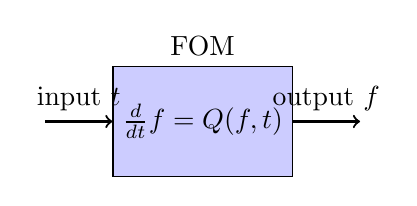
\begin{tikzpicture}[scale=0.5]
	\node [reco,label=FOM] (phys) {$\frac{d}{dt}f = Q(f,t)$};
	\draw [<-,thick] (phys)--+ (-4,0) node[midway,above] {input \(t\)};
	\draw [->,thick] (phys)--+ (4,0) node[midway,above] {output $f$};
\end{tikzpicture}

		\subcaption{Evolving the BGK-model in the Sod shock tube in time is generated through evaluating the FOM in space \(x\), velocity \(v\) and time \(t\), which yields the solution \(f(x,v,t)\). The operator \(Q\) is here the FOM described in \cref{Ch:BGK}.}
	\end{subfigure}\hfill
	\begin{subfigure}{.45\textwidth}
		\centering
		\tikzstyle{reco} = [rectangle,minimum height=4em,text centered, fill=blue!20,draw=black]
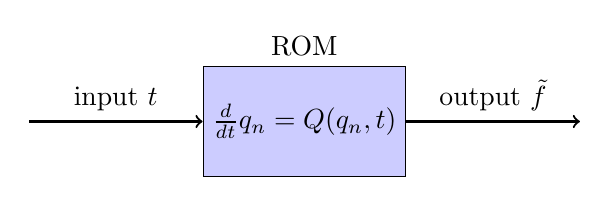
\begin{tikzpicture}[auto]
	\node [reco,label=ROM] (red) {$\frac{d}{dt}q_n = Q(q_n,t)$};
	\draw [<-,thick] (red)--+ (-3.5,0) node[midway,above] {input \(t\)};
	\draw [->,thick] (red)--+ (3.5,0) node[midway,above] {output $\tilde{f}$};
\end{tikzpicture}

		\subcaption{Evolving the ROM of the BGK-model in the Sod shock tube in time through evaluating the ROM at \(n\) and \(\mu_i\), yields an approximation to the FOM solution \(\tilde{f}\). The operator \(Q\) is here either POD or a neural network described in \cref{Ch:DimRedAl}.}
	\end{subfigure}
	\caption{Outline of the correlation between the FOM solution and the approximation obtained from the ROM.}
\end{figure}
MOR is partitioned into two successive phases called the \textit{offline} - and the \textit{online} phase. During the offline phase \textit{snapshots} of a dynamical-system are generated through experiments or simulations of the full order model (FOM). The snapshots \(U = \{u(t1),...,u(t_n)\}\) are created once, each representing one moment in time of the dynamical system. Thus in our case one needs a snapshot database of solutions \(f(x,v,t)\) of the BKG-model in the Sod shock tube. Next a mapping \(q_n\) is constructed such that \(\tilde{u} = q_n(u)\), for which \(u(t_i) \approx \tilde{u}(t_i)\), reducing the dimensionality of the FOM solution as outlined before. During the online phase the reduced order model is evaluated and the error is estimated by eg. \(||u(t) - \tilde{u}(t)||\). Therefore the online phase may be described as a stage of independence from the full order model.
Following \cite{ohlberger2015reduced} and \cite{Carlberg}, the success when building a ROM through linear reduction methods like the POD \cref{Sec: POD}, depends on a rapidly decaying Kolmogorov N-width. In particular advection dominated problems exhibit a slow decay of the Kolmogorov N-width. Thus yielding a need for non-linear methods like autoencoders described in \cref{Sec:AE}. The Kolmogorov N-width is given by
\begin{equation}
	d_{V}(W):= \sup_{f \in W} \inf_{\tilde{f} \in V} ||f-\tilde{f}||
\end{equation}
and gives the worst best approximation error for elements of \(W\). The convergence behaviour of the Kolmogorov N-width for advection dominated problems, especially when jump conditions are involved as in the Sod shock tube \cref{Ch:BGK}, decays with
\begin{equation}
	d_n(W) \leq \frac{1}{2} n^{-1/2},
\end{equation}
where \(n\) denotes the number of RB or intrinsic variables. Note that hereafter we will solely use the term intrinsic variables. The relevance of this contribution, using non-linear methods for MOR in rarefied gas dynamics, was already implied in the beginning and now takes shape. The BGK-model in the sod shock tube describes an advection problem with jump discontinuities \cref{Ch:BGK}. Thus linear reduction methods should fail. We will see in the following, that this is only partly true, because the advection character as well as the formation of sharp shock fronts heavily depends on the rarefaction of the gas as depicted in \cref{Ch:BGK}.   
\section{Offline Phase}
\subsection{Full order BGK-model}\label{Sec: FOM}
The FOM is the 1D BGK-model in the Sod shock tube for two levels of rarefaction, gratefully provided by Julian K\"ollermeier and the Departement of Mathematics at the RWTH Aachen. The Sod shock tube is discretized in space \(x\) with 100 nodes, in velocity \(v\) with 40 nodes for 25 time steps in time \(t\), as presented in \cref{Tab:Setup} and \cref{Fig:SodProbSetup}.
\begin{table}[htp]
	\centering
	\caption{Problem setup for the BGK model in the Sod shock tube. The diaphragm is positioned at \(x_d=0.5025\). For \(x<x_d\) the gas is present, for \(x\geq x_d\) particles are absent.}
	\begin{tabular*}{15cm}{ @{\extracolsep{\fill}} c c c c @{} }
		\toprule
		Variable   & Number of nodes \(i\)&   Domain extension& Step size (uniform)\\   
		\hline
		\(x\) 		&	200&     [0.0025,0.9975]&	    0.00499\\
		\(v\)       &   40 &  		    [-10,10]&	    0.05128\\
		\(t\)   	&	25 &        	[0,0.12]&	      0.005\\
		\bottomrule
	\end{tabular*} \label{Tab:Setup}
\end{table}
One is a slip flow with \(Kn=0.01\), hereafter will be referred to as \(\rare\). For this kind of rarefaction level the common Navier-Stokes equations are not valid anymore. The other is a continuum flow with \(\Kn=0.00001\) for which the Navier-Stokes equations can be utilized. A detailed description can be found in \cref{Ch:BGK}. Hereafter the continuum flow will be referred to as \(\hy\). Note that both \(\hy\) and \(\rare\) are three dimensional tensors containing \(f(x,v,t)\).\\
The reduction algorithms, introduced in \cref{Ch:DimRedAl}, require a distinct reshaping of the input data before they can be used. The preprocessed matrix for the FCNN, \(\mae\), is shown in \cref{Eq:AE_matrix}. Each row of \(\mae\) contains a sample shown to the FCNN. In turn we aquire \(x_it_i=5000\) samples. The preprocessed matrix for the CNN, \(\mconv\), is shown in \cref{Eq:CNN_matrix}. We obtain \(v_i=40\) samples, each containing a matrix \(\pi_{CNN}^{x_i\times t_i}\) holding the information about \(f(x,t)\) for a fixed point in \(v\). POD uses the \(mae\) matrix or its transposition.\\
\begin{minipage}{.55\linewidth}
	\begin{equation}
	\mae = \begin{bmatrix}
	f(v_1,t_1,x_1)&\cdots &f(v_n,t_1,x_1) \\
	f(v_1,t_1,x_2)&\cdots &f(v_n,t_1,x_2) \\
	\vdots& \vdots & \vdots\\
	f(v_1,t_1,x_n)&\cdots &f(v_n,t_1,x_n)\\
	f(v_1,t_2,x_1)&\cdots &f(v_n,t_2,x_1)\\
	\vdots & \vdots & \vdots\\
	f(v_1,t_n,x_n)&\cdots &f(v_n,t_n,x_n)
	\end{bmatrix}
	\label{Eq:AE_matrix}
	\end{equation}
\end{minipage}%
\begin{minipage}{.45\linewidth}
	\begin{equation}
	\mconv= \begin{bmatrix}
	n_{Filters},&f(v_1,\textbf{t},\textbf{x})\\
	n_{Filters},&f(v_2,\textbf{t},\textbf{x})\\
	\vdots&\vdots\\
	n_{Filters},&f(v_n,\textbf{t},\textbf{x})
	\end{bmatrix}
	\label{Eq:CNN_matrix}
	\end{equation}
\end{minipage}\\
In the following a distinction between \(\mconv\) and \(\mae\) is omitted, when referring to the preprocessed matrices. However a distinction between the levels of rarefaction, namely \(\hy\) and \(\rare\), will be utilized as \(\mhy\) for the former and \(\mrare\) for the latter.
\subsection{Contructing the mapping}
\begin{figure}[!htbp]
\begin{subfigure}{.45\textwidth}
	% This file was created by tikzplotlib v0.9.6.
\begin{tikzpicture}

\begin{groupplot}[group style={group size=2 by 1, horizontal sep=1cm, vertical sep=2cm}]
\nextgroupplot[
log basis y={10},
tick align=outside,
tick pos=left,
x grid style={white!69.0196078431373!black},
xlabel={\(k\)},
xmin=-0.95, xmax=41.95,,
xtick style={color=black},
y grid style={white!69.0196078431373!black},
ylabel={\(\sigma\)},
ymin=2.86160392849359e-16, ymax=240.32740800328,
ymode=log,
ytick style={color=black},
ytick={1e1,1e-3,1e-11,1e-15},
width=.55\textwidth,
height=.7\textwidth,
y label style={yshift=-2.5em},
grid=both
]
\addplot [semithick, red, mark=o, mark size=2, mark options={solid}]
table {%
1 36.8185958349281
2 5.78483852846218
3 2.9488881352441
4 1.08115123432794
5 0.4715894924307
6 0.27551553286601
7 0.155493855631619
8 0.0601331453526982
9 0.05155511017701
10 0.0132542951500055
11 0.0118122790965581
12 0.00208495452053553
13 0.00184461993287337
14 0.000261109297076443
15 0.000174118703867616
16 2.59262125849959e-05
17 1.30752219185821e-05
18 1.92140998809572e-06
19 9.1685066176197e-07
20 1.08651788755093e-07
21 5.26354986735524e-08
22 4.52124036969183e-09
23 2.44729256168519e-09
24 1.43747068296607e-10
25 9.28350136149776e-11
26 3.39879764456285e-12
27 2.74182349854538e-12
28 6.4789443879917e-14
29 6.12293316992491e-14
30 1.6313694307166e-14
31 2.92181471455653e-15
32 2.92181471455653e-15
33 2.92181471455653e-15
34 2.92181471455653e-15
35 2.92181471455653e-15
36 2.92181471455653e-15
37 2.92181471455653e-15
38 2.92181471455653e-15
39 2.92181471455653e-15
40 1.8678655154319e-15
};

\nextgroupplot[
tick align=outside,
tick pos=left,
x grid style={white!69.0196078431373!black},
xlabel={\(k\)},
xmin=-0.95, xmax=41.95,
xtick style={color=black},
y grid style={white!69.0196078431373!black},
ylabel={cusum-e},
ymin=0.760859233580134, ymax=1.0113876555438,
ytick style={color=black},
ytick={1,.8},
width=.55\textwidth,
height=.7\textwidth,
y label style={yshift=-2em},
grid=both
]
\addplot [semithick, red, mark=o, mark size=2, mark options={solid}]
table {%
1 0.772246889123937
2 0.893580238655189
3 0.95543131247198
4 0.978107779579132
5 0.987999072557982
6 0.993777837563443
7 0.997039223381299
8 0.998300478281949
9 0.999381814290284
10 0.999659814794242
11 0.999907569918492
12 0.999951300528145
13 0.99998999027099
14 0.999995466874262
15 0.999999118904556
16 0.999999662690558
17 0.999999936935114
18 0.99999997723548
19 0.999999996465846
20 0.999999998744749
21 0.999999999848745
22 0.999999999943575
23 0.999999999994906
24 0.999999999997921
25 0.999999999999868
26 0.999999999999939
27 0.999999999999997
28 0.999999999999998
29 0.999999999999999
30 1
31 1
32 1
33 1
34 1
35 1
36 1
37 1
38 1
39 1
40 1
};
\addplot [thick, , mark=x,black, mark size=2, mark options={solid}]
table{%
6 0
6 0.993777837563443
6 1.3
};
\end{groupplot}
\end{tikzpicture}


	\subcaption{Sigular values \(\sigma\) over \(k\) number of singular values left and \(cumultative\) \(energy\) over \(k\) right for the gas flow in the rarefied regime.}
	\label{Fig:CumSum_Rare}
\end{subfigure}\hfill
\begin{subfigure}{.45\textwidth}
	% This file was created by tikzplotlib v0.9.6.
\begin{tikzpicture}

\begin{groupplot}[group style={group size=2 by 1, horizontal sep=1cm, vertical sep=2cm}]
\nextgroupplot[
log basis y={10},
tick align=outside,
tick pos=left,
x grid style={white!69.0196078431373!black},
xlabel={\(k\)},
xmin=-0.95, xmax=41.95,,
xtick style={color=black},
y grid style={white!69.0196078431373!black},
ylabel={\(\sigma\)},
ymin=2.86160392849359e-16, ymax=240.32740800328,
ymode=log,
ytick style={color=black},
ytick={1e1,1e-3,1e-11,1e-15},
width=.55\textwidth,
height=.7\textwidth,
y label style={yshift=-2.5em},
grid=both
]
\addplot [semithick, red, mark=o, mark size=2, mark options={solid}]
table {%
1 36.8185958349281
2 5.78483852846218
3 2.9488881352441
4 1.08115123432794
5 0.4715894924307
6 0.27551553286601
7 0.155493855631619
8 0.0601331453526982
9 0.05155511017701
10 0.0132542951500055
11 0.0118122790965581
12 0.00208495452053553
13 0.00184461993287337
14 0.000261109297076443
15 0.000174118703867616
16 2.59262125849959e-05
17 1.30752219185821e-05
18 1.92140998809572e-06
19 9.1685066176197e-07
20 1.08651788755093e-07
21 5.26354986735524e-08
22 4.52124036969183e-09
23 2.44729256168519e-09
24 1.43747068296607e-10
25 9.28350136149776e-11
26 3.39879764456285e-12
27 2.74182349854538e-12
28 6.4789443879917e-14
29 6.12293316992491e-14
30 1.6313694307166e-14
31 2.92181471455653e-15
32 2.92181471455653e-15
33 2.92181471455653e-15
34 2.92181471455653e-15
35 2.92181471455653e-15
36 2.92181471455653e-15
37 2.92181471455653e-15
38 2.92181471455653e-15
39 2.92181471455653e-15
40 1.8678655154319e-15
};

\nextgroupplot[
tick align=outside,
tick pos=left,
x grid style={white!69.0196078431373!black},
xlabel={\(k\)},
xmin=-0.95, xmax=41.95,
xtick style={color=black},
y grid style={white!69.0196078431373!black},
ylabel={cusum-e},
ymin=0.760859233580134, ymax=1.0113876555438,
ytick style={color=black},
ytick={1,.8},
width=.55\textwidth,
height=.7\textwidth,
y label style={yshift=-2em},
grid=both
]
\addplot [semithick, red, mark=o, mark size=2, mark options={solid}]
table {%
1 0.772246889123937
2 0.893580238655189
3 0.95543131247198
4 0.978107779579132
5 0.987999072557982
6 0.993777837563443
7 0.997039223381299
8 0.998300478281949
9 0.999381814290284
10 0.999659814794242
11 0.999907569918492
12 0.999951300528145
13 0.99998999027099
14 0.999995466874262
15 0.999999118904556
16 0.999999662690558
17 0.999999936935114
18 0.99999997723548
19 0.999999996465846
20 0.999999998744749
21 0.999999999848745
22 0.999999999943575
23 0.999999999994906
24 0.999999999997921
25 0.999999999999868
26 0.999999999999939
27 0.999999999999997
28 0.999999999999998
29 0.999999999999999
30 1
31 1
32 1
33 1
34 1
35 1
36 1
37 1
38 1
39 1
40 1
};
\addplot [thick, , mark=x,black, mark size=2, mark options={solid}]
table{%
6 0
6 0.993777837563443
6 1.3
};
\end{groupplot}
\end{tikzpicture}


	\subcaption{Sigular values \(\sigma\) over \(k\) number of singular values left and \(cumultative\) \(energy\) over \(k\) right for the gas flow in the hydrodynamic regime.}
	\label{Fig:CumSum_Hydro}
\end{subfigure}
\end{figure}
\begin{table}[!htbp]\centering
\begin{tabular}{ |c|c|c|c|c|c|c|c|c| }
	\hline
	Intrinsic variables  & 3 & 4 & 5 & 6 & 7 & 8 & 9 & 10 \\ %[.5ex]
	\hline
	Error & 0.0327 & 0.0153 & 0.0087 & 0.0046 & 0.0021 & 0.0014 & 0.0005 & 0.0003\\ \hline
\end{tabular}
\caption{L2-Error for different numbers of intrinsic variables for the rarefied gas flow. Calculations with two intrinsic variables are also performed, but not shown here because two intrinsic variables is considered trivial.}
\label{Tab:Intrinsic units svd rare}
\end{table}
\begin{table}[!htbp]\centering
	\begin{tabular}{ |c|c|c|c|c|c|c|c|c| }
		\hline
		Intrinsic variables  & 3 & 4 & 5 & 6 & 7 & 8 & 9 & 10 \\ %[.5ex]
		\hline
		Error & 0.0205 & 0.0081 & 0.0030 & 0.0013 & 0.0006 & 0.0002 & 6.2\(e^{-5}\) & 2.7\(e^{-5}\)\\ \hline
	\end{tabular}
	\caption{L2-Error for different numbers of intrinsic variables for the hydrodynamic gas flow. Calculations with two intrinsic variables are also performed, but not shown here because two intrinsic variables is considered trivial.}
	\label{Tab:Intrinsic units svd hydro}
\end{table}
\textbf{}\subsection{Online Phase}
loremipsu
\subsection{Reduced Order Model}\label{Reduced Order Model}
The compression of the input data $y_0$ yields a code $C \in \mathbb{R}^{ix5000}$, composed  of the instrinsic variables \(c_i\). The index \(i\) corresponds to the i-th intrinsic variable whereas their number is given by the input data. Each of them describes the transport of a discontinuity as seen in \cref{Fig:Code_Fully}. Hence the expolitability of the code in terms of constructing a ROM is not provided. On that account the method of characteristics \cite{Dret2016} provides a means to bypass this shortage. It is necessary for $c_i(x,t)$ to satisfy the conservative condition \cref{Eq. Mass_Const} and the transport equation \cref{Eq. Transport}.\\
\noindent\begin{minipage}{.5\linewidth}
	\begin{equation}
	\frac{d}{dt}\int c_i\ dx = \frac{d}{dt}f_i = const. \label{Eq. Mass_Const}
	\end{equation}
\end{minipage}%
\begin{minipage}{.5\linewidth}
	\begin{equation}
	\frac{\partial}{\partial t}c_i + \frac{\partial}{\partial x}f_i = 0 \label{Eq. Transport}
	\end{equation}
\end{minipage}
The characteristics $u_i$ describe the constant transport velocities for each variable $c_i$ calculated using \cref{Eq. Characteristics}. Subsequently enabling the usage of a simple plynomial interpoaltion of any degree. Furthermore a linear mapping \(A_ix_i=c_i\) can be applied for the reconstruction of interpolated code variables \(\hat{c}_i\). \Cref{Fig. Flowchart} depicts this approach in detail.\\
Questions concering the capacity of this ROM, e.g. how many samples \(\hat{n}_t\) are needed to reconstruct \(n_t\) timestamps, are analysed in \cref{Results}.
\begin{equation}
	u_i = \frac{f_i(c^-_i) - f_i(c^+_i)}{c^-_i - c^+_i}
	\label{Eq. Characteristics}
\end{equation}
\begin{figure}
	\centering
	\usetikzlibrary{matrix}
\usetikzlibrary{shapes,snakes}
	\tikzstyle{rec} = [rectangle, rounded corners, minimum width=1cm, minimum height=1cm,text centered, draw=black]
	\tikzstyle{circ} = [circle,minimum size =1.5cm,text centered, draw=black]
	\tikzstyle{arrow} = [thick,->,>=stealth]
		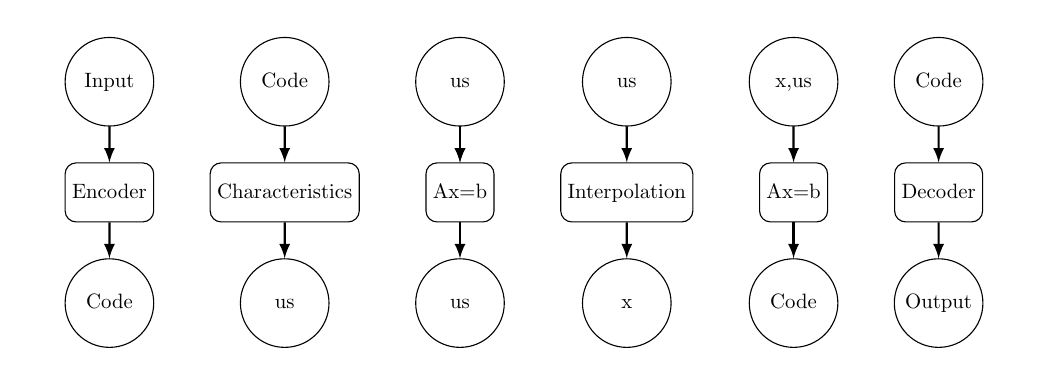
\begin{tikzpicture}[>=latex,text height=1.5ex,text depth=0.25ex,scale=.5,every node/.style={scale=0.75}]
		\matrix[matrix of nodes,column sep= 1em,row sep= 3ex]{
			&
			\node[circ] (1) {Input};&
			&
			\node[circ] (4) {Code};&
			&
			\node[circ] (7) {us};&
			&
			\node[circ] (10) {us};&
			&
			\node[circ] (13) {x,us};&
			&
			\node[circ] (16) {Code};&
			\\
			&
			\node[rec] (2) {Encoder};&
			&
			\node[rec] (5) {Characteristics};&
			&
			\node[rec] (8) {Ax=b};&
			&
			\node[rec] (11) {Interpolation};&
			&
			\node[rec] (14) {Ax=b};&
			&
			\node[rec] (17) {Decoder};&
			\\
			&
			\node[circ] (3) {Code};&
			&
			\node[circ] (6) {us};&
			&
			\node[circ] (9) {us};&
			&
			\node[circ] (12) {x};&
			&
			\node[circ] (15) {Code};&
			&
			\node[circ] (18) {Output};&
			\\
		};
	\path[->]
		(1) edge[thick] (2)
		(2) edge[thick] (3)
		(4) edge[thick] (5)
		(5) edge[thick] (6)
		(7) edge[thick] (8)
		(7) edge[thick] (8)
		(8) edge[thick] (9)
		(10) edge[thick] (11)
		(11) edge[thick] (12)
		(13) edge[thick] (14)
		(14) edge[thick] (15)
		(16) edge[thick] (17)
		(17) edge[thick] (18);
\end{tikzpicture}
	\caption{This figure shows the steps for obtaining a reduced oder model (ROM). Decoder and Encoder need to be used after training. In step one $y_0$ is the original input data, $C$ is the Code. In step two $c_i$ is the i-th intrinsic variable and $u_i$ the correspnding characteristic. The eigenvalue problem in step 3 outputs $x_i$ the eigenvector of A, a diagonal matrix composed of $u_i$ and b is the corresponing i-th intrinsic variable $c_i$. In step 4 $\hat{u}_i$ is the interpolated vector to $u_i$. Step 5 solves the linear equation for the diagonal matrix A composed of $\hat{u}_i$ times the eigenvector $x_i$ of the eigenvalueproblem in step 3. The output is $\hat{c}_i$ the i-th intrinsic variable corresponding to $\hat{u}_i$ the i-th interpolated characteristic.}
	\label{Fig. Flowchart}
\end{figure}